\documentclass[tikz,border=8pt]{standalone}
\usepackage[utf8]{inputenc}
\usepackage[OT4,plmath]{polski}
\usepackage{amsmath,amssymb}
\begin{document}
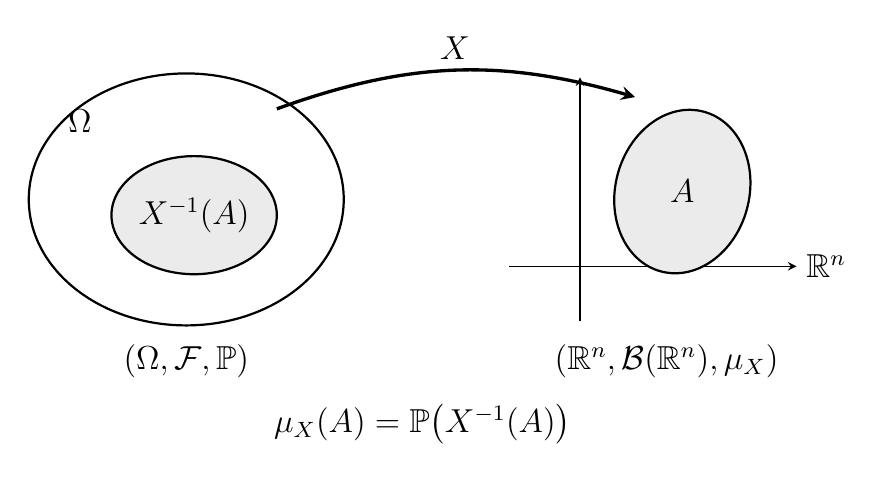
\begin{tikzpicture}[>=stealth,font=\large]
  \draw[thick] (0,0) ellipse (2cm and 1.6cm);
  \node at (-1.35,1) {$\Omega$};
  \draw[thick,fill=black!8] (.1,-.2) ellipse (1.05cm and .75cm);
  \node at (.1,-.2) {$X^{-1}(A)$};
  \node at (0,-2.05) {$(\Omega,\mathcal F,\mathbb P)$};
  \draw[->] (5,-1.55)--(5,1.55);
  \draw[->] (4.1,-.85)--(7.75,-.85);
  \node[right] at (7.75,-.85) {$\mathbb R^n$};
  \draw[thick,fill=black!8,rotate around={-15:(6.3,.1)}]
    (6.3,.1) ellipse (.85cm and 1.05cm);
  \node at (6.3,.1) {$A$};
  \draw[->,very thick] (1.15,1.15) to[bend left=18]
    node[above] {$X$} (5.7,1.3);
  \node at (6.1,-2.05) {$(\mathbb R^n,\mathcal B(\mathbb R^n),\mu_X)$};
  \node at (3,-2.85) {$\mu_X(A)=\mathbb P\bigl(X^{-1}(A)\bigr)$};
\end{tikzpicture}
\end{document}
